\section{Marco teórico y trabajos relacionados}
\subsection{Gestión de Horarios Académicos y Algoritmos de Optimización}
Imagina que eres un director de colegio y tienes que armar el horario de clases para cientos de estudiantes y profesores. Antes, esto se hacía con papel y lápiz, anotando manualmente quién da qué clase, cuándo y dónde, lo que tomaba días y generaba errores como superposiciones o aulas ocupadas al mismo tiempo. Hoy, sistemas como SGH automatizan esto usando algoritmos que resuelven estos conflictos de manera inteligente.

Un sistema de gestión de horarios académicos, como SGH, combina herramientas simples para registrar cursos, asignaturas, profesores y sus horarios disponibles, con algoritmos que generan horarios evitando choques. Es como un rompecabezas gigante donde cada pieza (clase, profesor, aula) debe encajar sin solaparse. En la práctica, soluciones similares usan algoritmos de optimización para resolver estos problemas, demostrando que es posible hacer esto de forma eficiente en entornos educativos \cite{saltos2022}. Comparado con métodos manuales tradicionales, que dependen de la intuición humana y son propensos a errores, SGH ofrece una alternativa automatizada que ahorra tiempo y reduce frustraciones.

\begin{figure}[h]
    \centering
    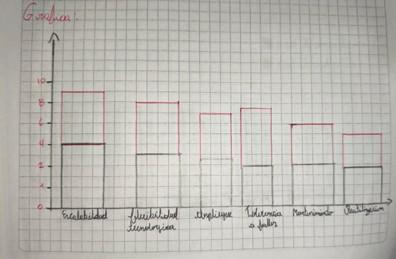
\includegraphics[width=0.4\textwidth]{graphics/estudio sobre metodologias de desarrollo y su impacto en la productividad.png}
    \caption{Estudio sobre metodologías de desarrollo y su impacto en la productividad}
    \label{fig:estudio}
\end{figure}

\subsection{Especificación de Requerimientos en Entornos Ágiles}
Cuando desarrollas software, necesitas saber exactamente qué quieres construir. En enfoques tradicionales, esto se hace con documentos largos y detallados que describen cada función paso a paso, como un manual de instrucciones. Pero en entornos ágiles, como el usado en SGH, se prefiere algo más flexible: historias de usuario.

Las historias de usuario son como pequeñas anécdotas que cuentan qué necesita el usuario. Según Izaurralde (2013), los requerimientos se dividen en funcionales (lo que hace el sistema) y no funcionales (como rapidez o seguridad). La ingeniería de requerimientos implica recopilar, analizar y validar estas necesidades, asegurando que sean correctas, completas y fáciles de cambiar si algo cambia.

\begin{figure}[h]
    \centering
    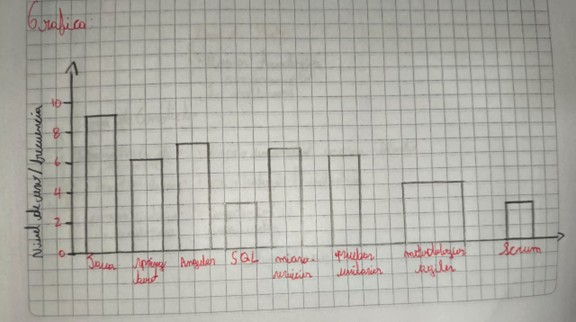
\includegraphics[width=0.4\textwidth]{graphics/practica de lenguaje de programacion java y nuevas tecnologias.png}
    \caption{Practicante en lenguaje de programación JAVA y nuevas tecnologias}
    \label{fig:java}
\end{figure}

En SGH, usamos historias de usuario porque permiten adaptar el sistema a medida que aprendemos más sobre las necesidades reales de los usuarios, en lugar de atarnos a un plan rígido desde el inicio. Comparado con especificaciones tradicionales, que pueden ser abrumadoras y difíciles de actualizar, las historias de usuario hacen el proceso más conversacional y humano, facilitando la colaboración entre desarrolladores y usuarios.

\subsection{Metodologías Ágiles: Scrum en SGH}
Scrum es como un juego de equipo donde divides el trabajo en rondas cortas llamadas sprints, cada una de unas semanas, para construir el software poco a poco. En SGH, adoptamos Scrum porque permite responder rápidamente a cambios, como cuando un profesor pide ajustar su disponibilidad.

En Scrum, los requerimientos se especifican con historias de usuario, que son simples y enfocadas en el valor para el usuario \cite{izaurralde2013}. A diferencia de métodos tradicionales que requieren planear todo al detalle antes de empezar, Scrum permite empezar con lo básico y refinar en cada sprint mediante reuniones diarias y retrospectivas. Esto hace que el desarrollo sea más adaptable y menos estresante.

\begin{figure}[h]
    \centering
    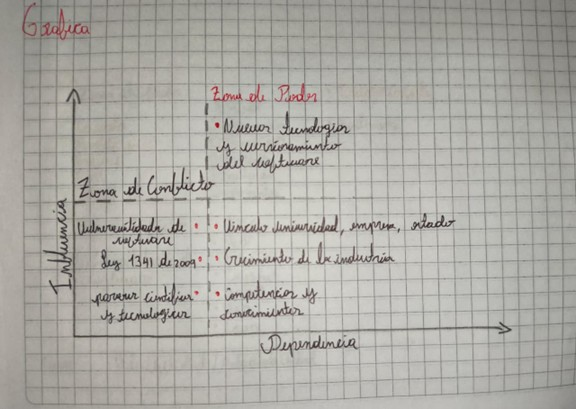
\includegraphics[width=0.4\textwidth]{graphics/analisis prospectivo de la industria de desarrollo de software en colombia.png}
    \caption{Análisis prospectivo de la industria de desarrollo de software en Colombia}
    \label{fig:analisis}
\end{figure}

\begin{figure}[h]
    \centering
    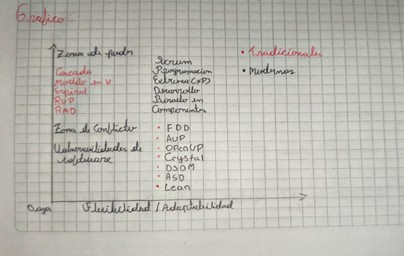
\includegraphics[width=0.4\textwidth]{graphics/una revision comparativa de la literatura acerca de metadologias tradicionales y modernas de desarrolladores de software.png}
    \caption{Una revisión comparativa de la literatura acerca de metodologías tradicionales y modernas de desarrollo de software}
    \label{fig:revision}
\end{figure}

Comparado con enfoques waterfall (donde todo se planea de una vez), Scrum en SGH es como construir una casa habitación por habitación en lugar de diseñar todo el plano primero: puedes ajustar si encuentras un problema, y el resultado final se siente más vivo y útil.



\subsection{Tecnologías Backend: Java con Spring Boot}
El corazón de SGH es su backend, construido con Java y Spring Boot. Java es como un lenguaje confiable y maduro, usado en muchas aplicaciones grandes porque es rápido, seguro y funciona en cualquier máquina. Spring Boot simplifica el desarrollo al proporcionar herramientas listas para usar, como manejar bases de datos o seguridad.

En SGH, usamos JPA para conectar el código con la base de datos de forma automática, y Spring Security con JWT para autenticar usuarios de manera segura. Comparado con otros frameworks como Node.js o Python Django, Spring Boot ofrece más estabilidad para aplicaciones complejas, aunque puede ser un poco más pesado al inicio. Pero para un sistema como SGH, que maneja datos sensibles de horarios, esta robustez es clave.

\begin{figure}[h]
    \centering
    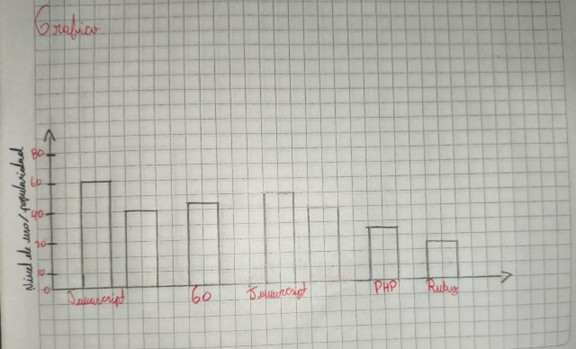
\includegraphics[width=0.4\textwidth]{graphics/tecnologias frontend y backend en tendencia.png}
    \caption{Tecnologías Front-end y Back-end en Tendencia}
    \label{fig:tecnologias}
\end{figure}



\subsection{Bases de Datos: MySQL en SGH}
Las bases de datos son como el archivador digital donde guardas toda la información. MySQL es una opción popular porque es gratuita, rápida y fácil de usar, ideal para proyectos como SGH que necesitan almacenar relaciones complejas, como qué profesor da qué clase en qué aula \cite{lozano2018}.

MySQL surgió en los 90 como una evolución de sistemas más antiguos, y hoy es una herramienta clave para datos estructurados. Comparado con bases de datos no relacionales como MongoDB, que son más flexibles para datos irregulares pero pueden ser menos consistentes, MySQL garantiza que todo esté bien organizado con el modelo ACID \cite{saltos2022}. En SGH, optamos por MySQL porque nuestros datos (cursos, profesores, horarios) tienen relaciones claras que necesitan integridad, y lo ejecutamos en XAMPP para desarrollo local, con phpMyAdmin para gestionar todo sin complicaciones.

\subsection{Interfaces Web y Móviles: Frameworks para Android}
SGH no es solo un sitio web; también tiene una app móvil para Android. Para lograr esto, usamos React Native, que permite desarrollar una app nativa para Android con un solo código base. En el frontend web, Next.js con Tailwind CSS crea interfaces modernas y responsivas.

Comparado con desarrollo nativo puro (escribir código específico para Android), React Native ahorra tiempo y dinero, aunque a veces requiere ajustes para un rendimiento óptimo. En SGH, esto significa que estudiantes y profesores pueden acceder a sus horarios desde dispositivos Android, haciendo el sistema más accesible y práctico.

\subsection{Arquitectura Modular y Microservicios}
La arquitectura de SGH es modular, como construir con bloques Lego: cada parte (backend, frontend, móvil) es independiente, pero encaja perfectamente. Esto facilita mantener y expandir el sistema, como agregar nuevas funciones sin romper lo existente.

Comparado con arquitecturas monolíticas (todo en un bloque grande), la modularidad en SGH permite actualizaciones más seguras y escalabilidad. La coexistencia de requerimientos tradicionales con historias de usuario asegura que tengamos lo mejor de ambos mundos: precisión y flexibilidad \cite{izaurralde2013}.

\begin{figure}[h]
    \centering
    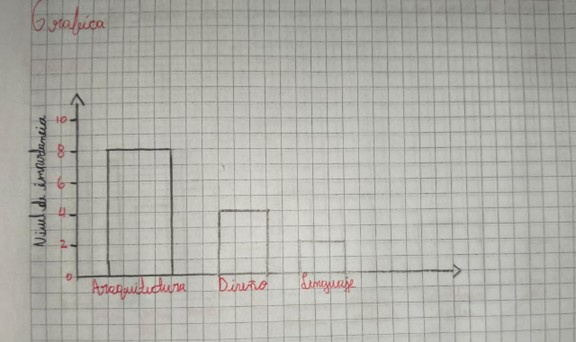
\includegraphics[width=0.4\textwidth]{graphics/Especificando una arquitectura de software.png}
    \caption{Especificando una arquitectura de software}
    \label{fig:arquitectura}
\end{figure}



\subsection{APIs RESTful y Autenticación JWT}
Las APIs son como puentes que conectan las partes de SGH. Usamos RESTful para intercambiar datos de forma segura y eficiente, con JWT para autenticar usuarios sin guardar sesiones en el servidor \cite{cein2025}.

Comparado con APIs más antiguas, REST es simple y escalable, ideal para apps móviles. En SGH, documentamos todo con Swagger para que sea fácil probar y entender, mejorando la colaboración entre equipos.

\subsection{Docker: Contenerización para Despliegue}
Docker es como empaquetar SGH en una caja portable que funciona igual en cualquier máquina. Resuelve problemas de compatibilidad, reduciendo tiempos de despliegue de días a horas (Chamú, 2025).

Comparado con máquinas virtuales, que simulan computadoras completas, Docker es más ligero y eficiente, perfecto para orquestar servicios en SGH sin complicaciones.

